\section{Discussion}
As can be seen, our approach only provides a noticeable improvement to the performance of Cassandra when multiple nodes in the cluster are heavily loaded. This is not what we initially imagined our results would be. One of our intuitions is that the performance decrease exists because the resource usage formula does not accurately reflect what the time to execute a query will be. To confirm this intuition we performed an experiment that compared the resource usage to the query execution time in a Cassandra instance.

In the remainder of this section we will provide what we feel will be a more accurate resource usage formula for distributed databases, as well as discuss several limitations that may also have affected our work.

\subsection{Re-examining the Resource Usage formula}

\begin{figure}[t]
\centering
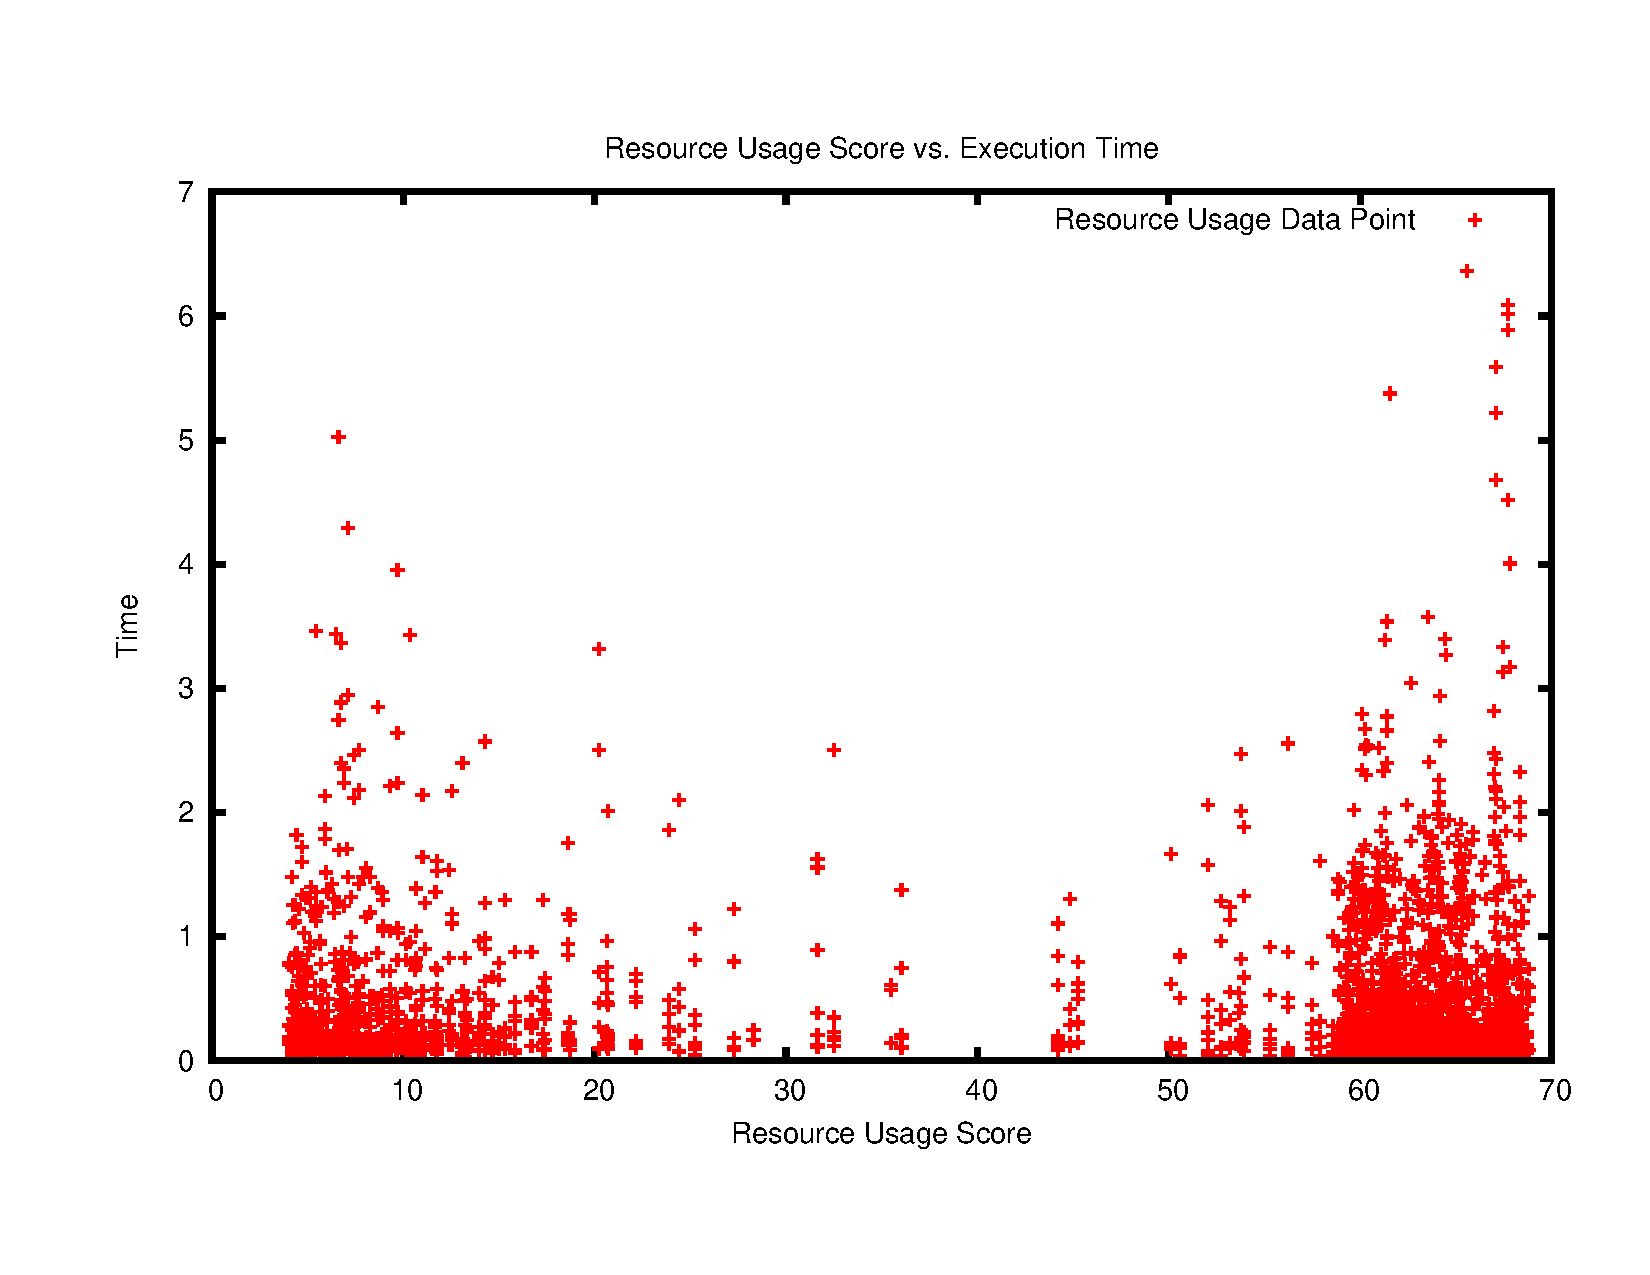
\includegraphics[scale=0.3]{images/ResUse.pdf}
\vspace{-15pt}
\caption{The experimental results comparing the resource usage score to the query execution time.}
\label{fig:resourceUsageFig}
\end{figure}

To examine how representative the resource usage score is we have performed an experiment that compares resource usage to query execution time. The setup for the resource usage experiments is different than the setup for the primary experiments. This experiment was performed on a single Cassandra instance on a single machine with a 4-core 2.6Ghz processor and 8GB of memory. The server also contained a solid-state drive instead of the hard disk drive used in the servers in the cluster. The settings for YCSB and Cassandra were identical, except that the replication factor was set to \textit{one}.

The CPU usage and memory usage was recorded every 250ms, and the query execution time was recorded for each query. The queries that executed in that 250ms window had their execution time averaged. The CPU usage and memory usage were used to calculate the resource usage of the server for each 250ms interval. The results were gathered over a 300 second interval using 10 parallel YCSB clients. Given our previous results showing that even 1000 parallel clients did not heavily load the node servers we do not believe that the results would be any different for a number of parallel clients greater than 10.

The results from the experiment are shown in Figure~\ref{fig:resourceUsageFig}. There appears to be little correlation between the resource usage score and the query execution time. When the resource usage score is higher, there are slightly more outliers that require a longer execution time, but in most cases the execution time seems to be independent of the resource usage. In addition, the resource usage scores tend to either be very low or very high. While this experiment was running, we also periodically loaded the server with other work. This resulted in a higher resource usage score, but not in a higher query execution time.

This experiment seems to indicate that the current formula is not ideal for determining the resource usage of the server. However, we believe that this could still work if the formula was changed to reflect how some variables affect the query execution time much more.  Additional variables can also be added that affect query execution time. For example, one of the primary bottlenecks in any database system is the hard disk, and we do not consider any variables related to the disk (e.g., disk access throughput).

Something to note is that the heap memory of the Cassandra instance rarely exceeded 1GB. Meaning that the memory usage score had little effect during the normal experiments. Even when the server was being artificially loaded the heap memory therefore has little effect. This also means that little data is being cached, which increases the importance of measuring the disk load.

\subsection{Limitations}

\subsection{Future Work}

\section{Conclusion}
Because the code that handles scans is completely disjoint from the code that handles reads, writes or updates it is plausible to implement our algorithm purely for scans while losing very little performance (just the overhead of a single thread in Cassandra that queries the CJD for resource information).
